\section{Network integrated M2M-oriental polling service}
\label{sec:polling}
The main idea of our proposed service is: the network provides a list of polling periods. MTC devices register to network for an appropriate polling period by traditional random access procedure. 
% 拉格朗日说,这句话英语表述有问题 C'est pas claire, il y un problème englais,surtout tu suppose qu'on va allouer les ressources
Upon received requests, the eNB deterministically allocates RNTI and the phase number in the allocated polling period for each registered device.
% according to proposed algorithm (detailed in Sec.\ref{prposed_algorithm}). This coordination mechanism schedules all data transmissions without collision.
% Ce que nous allouons est justement le RNTI, mais ensuite, il n'y a pas d'allocation fixe. Donc je suggère de dire: il y a en fait deux modes, c'est à dire, on peut avoir semi-static allocation (on peut avoir une allocation vraiement de type circuit); ou alors on peut avoir flexible packet access  (flexible allocation): 
% 'There are two possible modes: the first is the semi-persistent allocation where a fixed resource is periodically allocated to a MTC device. ' The second possibity is flexible allocation, where the standard packet access is used by a window defined for this polling period a MTC device pass standard packet access  
Afterwards, both the eNB and devices monitor LTE frames to determine their respective actions. When a transmission condition is verified for a certain device, the eNB directly allocates radio resources for the latter to poll the data. The qualified device directly sends its data via allocated resource without collision with other devices. Note that the radio resource allocation for data transmission may be of two types: either a semi-persistent allocation by which a fixed resource is periodically allocated to the registered MTC devices, or a flexible allocation where a standard packet access is used within the allocated polling window (detailed in Sec.\ref{polling-window}). 
%For radio resource allocation when transmitting data, there exist two possibilities: one is semi-persistent allocation 
Therefore, our proposed service consists of periodic polling mechanism and RNTI allocation algorithm. 
In this section, we first introduce some important concepts for our proposal. Second, we detail the periodic polling mechanism. Third, we present the RNTI allocation algorithm. 
\subsection{Terminology Related to the Proposed Service }
% il faut aborder le fait qu'il y une correspondance entre PRD-RNTI et IMSI en fonction du temps... 
% Ce que nous allouons a mobile est une periode(polling period) et PRD-RNTI..
% 那拉格朗日的意思应该是 我们把polling period paging和给他分配的PRD-RNTI告诉手机啊。。。“Tu(un mobile) as telle period et telle PRD-RNTI quand le extened SFN modulo une variable. Il faut aussi preciser cette valeur...  Cela est indique par le reseau...”

% Quand un mobile se presente, il va demander une period. On va dire, OK, tu as telle periode et telle PRD-RNTI a tels moments. C'est quand le eSFN modulo une valeur 

%?“Comment le mobile sais quand il a ce PRD-RNTI???”
\subsubsection{LSFN}
\label{LSFN}
We propose to extend the frame counting mechanism of LTE known as SFN (System Frame Number) and define a counter called LSFN for Long SFN. It is used to help\begin{inparaenum}[i)]
	\item the eNB to determine which target it should poll for data 
	\item a device to determine whether it is its turn to transmit data.
\end{inparaenum}
 The necessity for this extension is due to the fact that conventional LTE SFN varies from $0$ to $1023$ and each SFN value repeats every $10.24$ sec. LSFN is constructed by extending $19$ bits as MSB (Most significant bit) for current SFN. The value of LSFN is reset when it reaches 14$\times$16875 $\times$1024. The period is thus 14$\times$16875$\times$1024$\times$10 ms, which is exactly $28$ days and allows to define any process with period up to about one month.
The 19 MSB of LSFN is broadcasted in a System Information Block every $10.24$ sec. 
The relationship between LSFN and SFN is shown in Fig.\ref{fig:construction of LSFN}.  
Note that the LSFN indexing system does not modify the SFN-based mechanisms. 
Terminals other than those of periodic MTC applications still access network through conventional random access and use current LTE SFN system. 

\begin{figure}[!t]
	\centering
	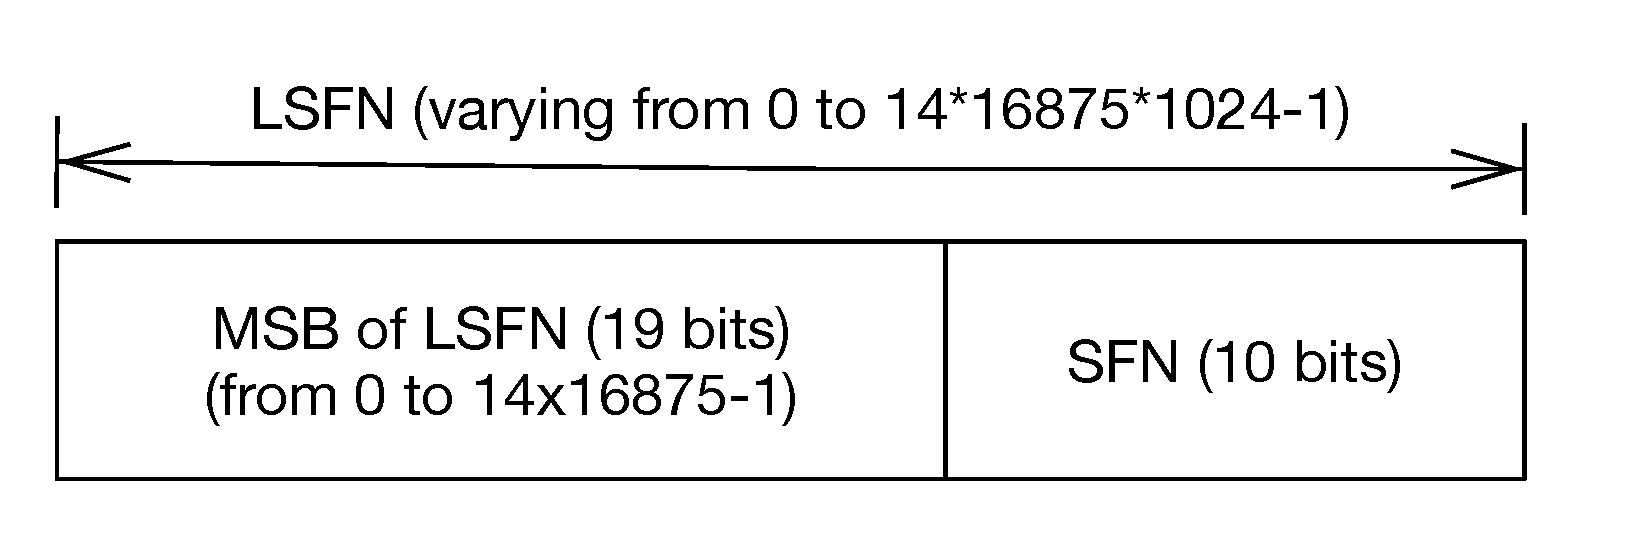
\includegraphics[width=0.6\linewidth]{Chapter6/Figures/Construction-LSFN.eps}
	\caption{Construction of LSFN}
	\label{fig:construction of LSFN}
\end{figure}

\subsubsection{PRD-RNTI}
\label{PRD-RNTI}
PRD-RNTI is a kind of RNTI used to uniquely identify one MTC device in a polling window (detailed in \ref{polling-window}).
The range FFF4-FFFC (marked as reserved for future use in \cite{3GPP/TS/36321}) is thus allocated as PRD-RNTI. 
%PRD-RNTI is reserved to a certain MTC device at the beginning of each polling window and released at the end of the same polling window then reallocated to the next polled MTC device. Network keeps a mapping table between PRD-RNTI and devices identity to consult which MTC device keeps which PRD-RNTI at a given moment. one PRD-RNTI can sequentially serve enormous MTC devices.
The same PRD-RNTI is allocated to several MTC devices but at different time. Hence, during a given period of time, the PRD-RNTI is allocated to only one device. As the allocation is deterministic, one device knows when it can use the PRD-RNTI and the network knows to which device the PRD-RNTI is used at any time. One PRD-RNTI can sequentially serve enormous MTC devices.

\subsubsection{{Polling period}}
\label{polling-period}
% 关于Polling period的notation是使用T_n还是T_p,n 让人伤脑筋啊
The polling period denoted by $T_n$ is the time interval between two consecutive eNB-triggered polling procedures for the same MTC device. It is computed from the application report period $T$ by:
\begin{align}
T_{n} = 2^{\floor{\log_2 \frac{T}{WT_f}}}\cdot W \cdot T_f =N_{n}\cdot W \cdot T_f\label{eq:period-conversion}
\end{align}
where $\floor{x}$ means the maximum integer not greater than $x$, $N_{n}$ is the number of polling window contained in period $T_{n}$, $W$ is the number of LTE frame, $T_{f}$ refers to LTE frame duration. As a network integrated service, the eNB uniquely supports polling periods satisfying (\ref{eq:period-conversion}). 
%Each user defined report period should be converted to an approximate polling period to use this network-integrated service. For example, a report period $300 s$ is converted to $204.8s$ as polling period.

% sur une period ou bien une interval du temps, il y a une correspondance entre mobile et RNTI

%\subsubsection{{Polling period}}
%\label{polling-period}
%% 关于Polling period的notation是使用T_n还是T_p,n 让人伤脑筋啊
%The polling period denoted by $T_n$ is the time interval between two consecutive eNB-triggered polling procedures for the same MTC device. It can be represented by the combination of three primes $2,3,5$. Namely, $T_n =  2^{a} \cdot 3^{b} \cdot 5^{c}$, where $a, b, c$ are the occurrence number of the corresponding prime. For a given $T$, we choose the closet $T_n$ to use polling service.
%\begin{align}
%T_{n} = 2^{a} \cdot 3^{b} \cdot 5^{c}\cdot W \cdot T_f\label{eq:period-conversion}
%\end{align}
%where $\floor{x}$ means the maximum integer not greater than $x$, $N_{n}$ is the number of polling window contained in period $T_{n}$, $W$ is the number of LTE frame, $T_{f}$ refers to LTE frame duration. As a network integrated service, the eNB uniquely supports polling periods satisfying (\ref{eq:period-conversion}). 

\subsubsection{Polling window}
\label{polling-window}
The polling window is a time interval which is reserved for data transmission of a unique MTC device. It is a configurable system parameter. Its duration is equal to $W$ LTE frame and should ensure that the device can deliver its data even in case of retransmission due to the HARQ mechanism.
The relationship between polling window and LTE frame is illustrated in Fig.\ref{fig:Illustration of Polling window in time domain}. 

\begin{figure}[!t]
	\centering
	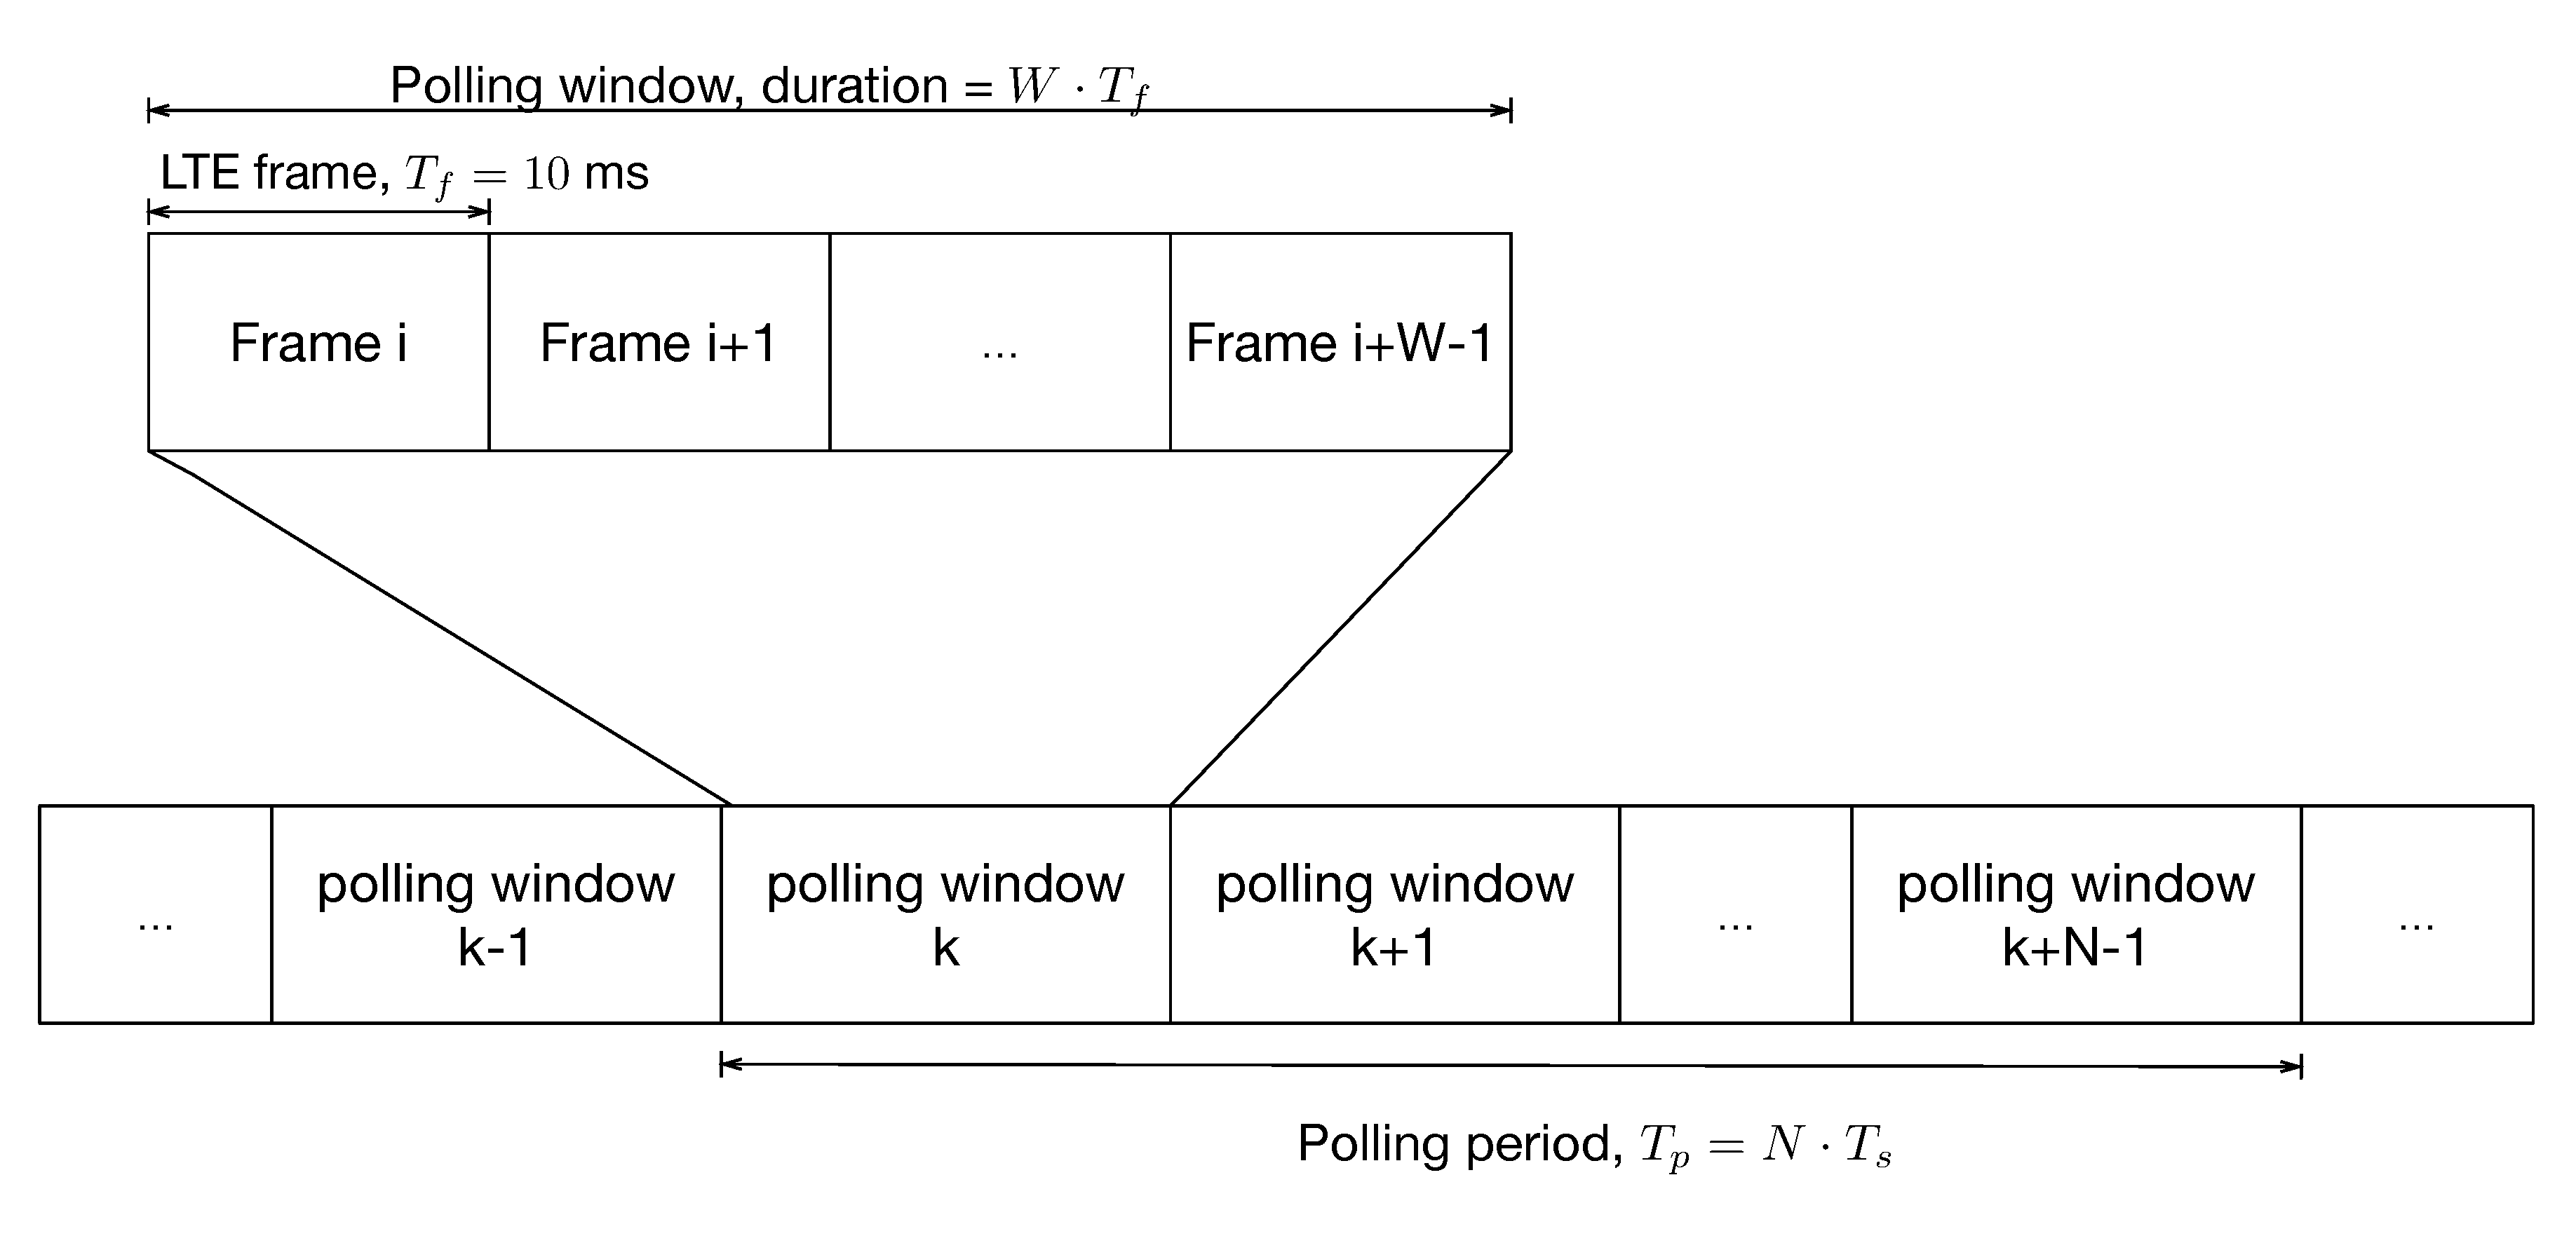
\includegraphics[width=0.9\linewidth]{Chapter6/Figures/Polling_window_illustration.eps}
	\caption{Illustration of Polling window in time domain}
	\label{fig:Illustration of Polling window in time domain}
\end{figure}

% 接下来讨论 polling window的长度 
%Supposing the maximum retransmission number is set as $3$, the worst case is that eNB receives report from device after four times transmission and takes in total 32 ms if each transmission takes $8$ ms. This analysis procedure is illustrated in 
%%8 ms for a transmission comes from where??
%in Fig.\ref{fig:UE Transmission and 3 Retransmission}. If taking into account possible eNB response to MTC device, a conversation including a report and response can be achieved in $64$ ms. Thus, we define in our proposal the duration of polling window as $100$ ms ($10$ LTE frames).
%\begin{figure}[htbp]
%	\centering
%	\includegraphics[width=10cm, height= 8cm ]{Figures/UE-Retransmission.png}
%	\caption{UE Transmission and 3 Retransmission}
%	\label{fig:UE Transmission and 3 Retransmission}
%\end{figure}

% 关于mobile是如何知道自己是在什么时候可以上传数据的设想:
% 方案一: 用户在购买SIM卡的时候,什么时候报告,分配什么PRD-RNTI都已经确定好了 然后输入到eNB的数据库里。。
% 方案二: 用户的设备的安放到 某个eNB管理下的小区的时候, 自己像eNB发出特设的信息(这岂不是还是有点儿类似于RA么),然后eNB会为其分配 指定的 上报时机以及 PRD-RNTI
% 个人感觉,拉格朗日所言更像是 方案二
\subsection{Multiple-period polling mechanism}
%Simply speaking, periodic polling mechanism refers to allocate resource to a certain MTC device at a given time. Since periodic MTC applications comportment is deterministic, we could define a deterministic rule for resource allocation for each device.

Different with traditional RACH method for network access, the eNB in our proposed periodic polling mechanism allocates system resource (i.e. RNTI) to a certain registered MTC device when LSFN satisfies some predefined rules, since periodic MTC application comportment is deterministic. It consists of two stages: registration stage and polling stage. 

\subsubsection{Registration stage} 
%在这个问题上,貌似拉格朗日跟我有分歧啊。。。
%我的想法是,device只是上报用户设置的 reporting period,由eNB负责conversion然后把确定好的 polling period下行给 device.
Let consider one MTC device $m$ asking for periodic polling service. It first sends a polling activation request including the polling period $T_n$ by traditional random access procedure. If the request is accepted, the network then sends back a confirmation message with \begin{inparaenum}[i)]
	\item the number of polling windows $N_n$ that corresponds to the polling period;
	\item a phase value $\phi _{m}$ between $0$ and $N_{n}-1$;
	\item a PRD-RNTI value.
\end{inparaenum}
Once the registration stage is finished, eNB updates its internal data for periodic polling service and registered device $m$ can use allocated PRD-RNTI with following rules: 
\begin{align}
&\textrm{PRD-RNTI for device $m$} \textrm{ when} \floor{\frac{LSFN}{W}}\bmod N_n=\phi _{m} \label{eq:rule}
\end{align}
%where $\floor{\frac{LSFN}{W}}$ means the maximum integer not great than $\frac{LSFN}{W}$.
\subsubsection{Periodic polling stage}
At this stage, for each LTE frame, the eNB manipulates LSFN value and determines current polling window is reserved for which MTC device by checking stored rules like in (\ref{eq:rule}). Still taking device $m$ as an example, once rule (\ref{eq:rule}) is satisfied, the eNB allocates radio resource for the device holding the PRD-RNTI, namely device $m$. As to device $m$, it also monitors the value of LSFN. If the MTC device has no specific action, it can switch to a low consumption mode in order to spare energy. As soon as rule (\ref{eq:rule}) is checked then the device $m$ listens to the PDCCH during all the polling window. It is up to the eNB to allocate uplink radio resource in order to allow the data transmission of the MTC device. Note that the PRD-RNTI is allocated to only one device during a given polling window. Standard system resource allocation mechanisms can be used without any risk of collision. This procedure is illustrated in the right part of Fig. \ref{fig:Comparison}.

Finally, Fig.\ref{fig:Comparison} illustrates the comparison between MTC device data report via conventional random access and our proposal.
%: In RACH mechanism, MTC device has to pass three transmission for reporting collected data while in our proposal it needs just one transmission.
%Unlike traditional random access method, for a already registered MTC device, it manipulates the $LSFN$ received in System Information. When the condition for its turn of transmission, it directly sends collected data with received PRD-RNTI in PDCCH channel without demanding resource allocation.

\begin{figure}[!t]
	\centering
	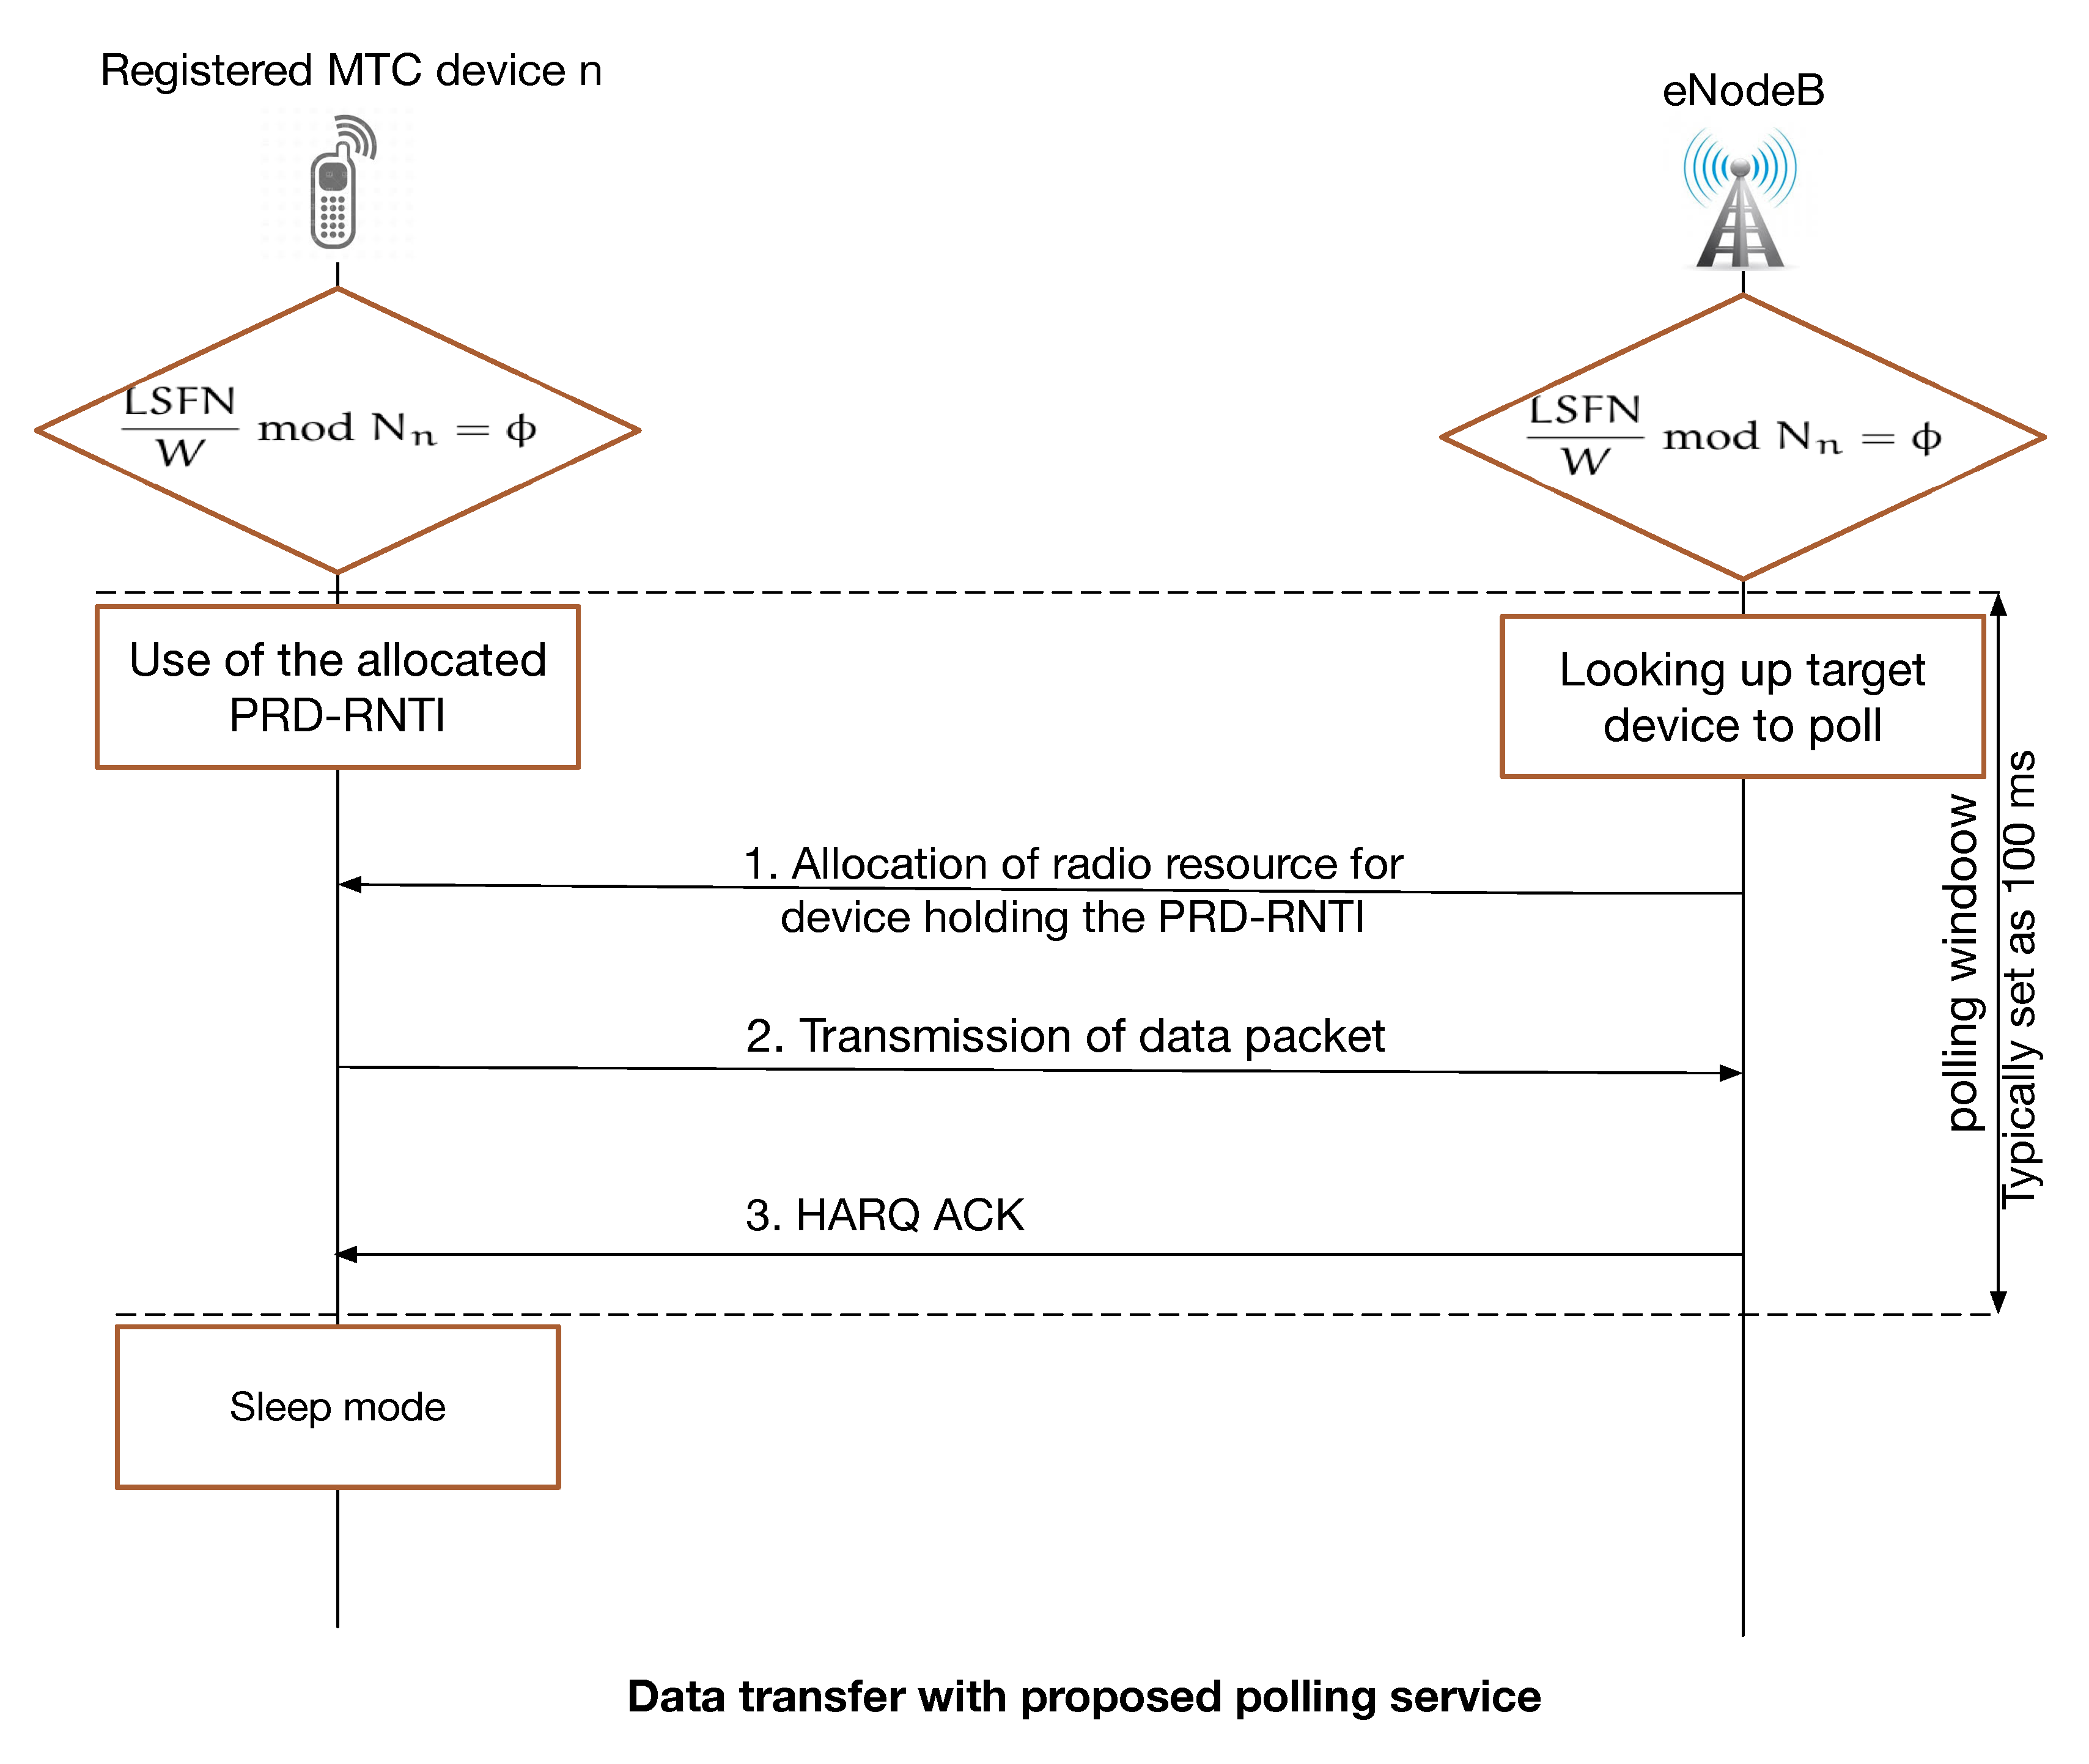
\includegraphics[width=\linewidth]{Chapter6/Figures/proposed-polling-service}
	\caption{Proposed polling service work flow}
	\label{fig:Comparison}
\end{figure}
\subsection{RNTI allocation algorithm}
\label{prposed_algorithm}
%As introduced in previous section, time domain resource is divided into a series of polling windows and eNB supports a group of polling periods. A resource allocation algorithm \ref{alg:resource-allocation-algo} is thus proposed to allocate polling windows for each registered MTC device. A detailed explanation about this algorithm is given in this section.

%When receiving all requests, our proposed resource allocation algorithm \ref{alg:resource-allocation-algo} is executed for allocating polling window, for each registered device. 
Algorithm (\ref{alg:resource-allocation-algo}) serves for allocating resource such as PRD-RNTI and phase value 
(refers to a series of polling windows) 
for each registered device.
Some notations about our algorithm: the eNB provides $N$ different polling periods denoted by $T_{n}$, where $n=0,1,...,N-1$ and $T_{n} = 2T_{n-1}$. The number of polling windows in polling period $T_{n}$ is denoted by $N_{n}$. All devices are regrouped into $N$ groups according to polling periods with ascending order. The number of devices waiting for polling window allocation in group $n$ is denoted by $g_{n}$. Each PRD-RNTI provides a limited number of polling windows. The cardinality of available polling windows set when allocating for devices in group $i$ is denoted by $C_{PRD-RNTI, i}$. When there are no available polling windows, a new PRD-RNTI should be taken from PRD-RNTI set. 
The algorithm (\ref{alg:resource-allocation-algo}) first takes an available PRD-RNTI and initiates $C_{PRD-RNTI, 0}$ as $N_{0}$. A loop structure from line \ref{algo: for-loop-all-groups} to \ref{algo: end-for-loop-all-groups} is used to process all requests on the basis of group. In iteration $i$ for phase value allocation of group $i$, algorithm first calculates available polling windows $C_{PRD-RNTI, i}$ by a recursive relation $C_{PRD-RNTI, i}=2C_{PRD-RNTI, i-1}$, since the number of polling window contained in a polling period $N_{i} = 2N_{i-1}$. If the number of devices remaining to be processed is still more than $0$, algorithm enters in while-loop (line \ref{algo:while-loop} to \ref{algo:end-while-loop}) for allocating each device a polling window. In this while-loop, first check if it needs take a new PRD-RNTI. Then algorithm calculates allocated phase value $\phi$ for $\min (g_{i}, C_{PRD-RNTI, i})$ devices then updates $C_{PRD-RNTI, i}$ and $g_{i}$. 
%The condition to exit this while-loop is satisfied when there is no devices in group $i$ to be allocated polling window.
\begin{algorithm}
	\caption{RNTI allocation algorithm} % Title of this algo
	\label{alg:resource-allocation-algo} % Facilitate reference for this algo
	\begin{algorithmic}[1] % 1 --> show lines number
		\Procedure{Allocation}{$g_{0}, g_{1}, g_{2}, ..., g_{N}$} 
		\State $PRD-RNTI \gets $ $pop$ $PRD-RNTI$ $set$
		\State $C_{PRD-RNTI, 0} \gets N_{0} $
		\For{$i=0$; $i<N$; $i++$ } \label{algo: for-loop-all-groups}
		\If {$i > 0$}
		\State $C_{PRD-RNTI, i} \gets 2C_{PRD-RNTI, i-1}$
		\EndIf
		\While{$g_{i} > 0 $} \label{algo:while-loop}
		\If {$C_{PRD-RNTI, i} = 0$}
		\State $PRD-RNTI \gets $ $pop$ $PRD-RNTI$ $set$
		\EndIf
		\For{$j=0$; $j<min(g_{i}, C_{PRD-RNTI, i})$; $j++$ } \label{algo:allocation-for-loop}
		\State $\phi _{j} \gets \floor{\frac{LSFN}{W}} \mod N_{n} $
		\EndFor \label{algo:end-allocation-for-loop}
		\State $C_{PRD-RNTI, i} \gets C_{PRD-RNTI, i}-\min (g_{i}, C_{PRD-RNTI, i})$
		\State $g_{i} \gets g_{i} - \min (g_{i}, C_{PRD-RNTI, i})$
		\EndWhile \label{algo:end-while-loop}
		\EndFor \label{algo: end-for-loop-all-groups}
		\EndProcedure
	\end{algorithmic}
\end{algorithm}

\subsection{An example}
Let take an example to illustrate the proposed RNTI allocation algorithm. 
Supposing an eNB supports $4$ different polling periods whose notations are $T_0 = 4T_s, T_1=8T_s, T_2=16T_s, T_3=32T_s$, $T_s$ is duration of a polling window. All devices are regrouped into four groups $0, 1, 2, 3$. Each group consists of two devices so $g_{0}=2, g_{1}=2,g_{2}=2,g_{3}=2$ and each device is respectively identified as $a_{0}, a_{1}, b_{0}, b_{1}, c_{0}, c_{1}, d_{0}, d_{1}$. 
To allocate polling window for these devices, first take value $FFF4$ from PRD-RNTI set. For group $0$ with polling period $4T_s$, the available polling windows is $N_{0}=4$. Allocate respectively polling windows satisfying $\phi_{a_{0}}=0, \phi_{a_{1}}=1$ for $a_{0}, a_{1}$. Since there are just two devices to be served in group $0$, it still remains $2$ polling windows after allocation. Then for group $1$, at this time available polling window number is $4$ , allocate polling windows satisfying $\phi_{b_{0}}=2, \phi_{b_{1}}=3$ for $b_{0}, b_{1}$. So after allocation for group $1$, $C_{PRD-RNTI, i=1}$ is updated as $2$. With the same philosophy, allocation for group $2, 3$. The RNTI and phase value allocation result is shown in Fig.\ref{fig:Illustration-Resource-Allocation} and resumed in Tab.\ref{tab:resume}.
\begin{table}[!t]
	\renewcommand{\arraystretch}{1.3}
	\caption{Polling window allocation resume}
	\label{tab:resume}
	\centering
	\begin{tabular}{ccccc}
		\hline
		group name & number of device& identity & polling period & phase value \\
		\hline
		\multirow{2}{*}{0} & \multirow{2}{*}{2} & \multirow{2}{*}{$4T_{s}$} & $a_{0}$ & $0$\\ &&& $a_{1}$ & $1$ \\
		\hline
		\multirow{2}{*}{1} & \multirow{2}{*}{2} & \multirow{2}{*}{$8T_{s}$} & $b_{0}$ & $2$\\ &&& $b_{1}$ & $3$ \\
		\hline
		\multirow{2}{*}{2} & \multirow{2}{*}{2} & \multirow{2}{*}{$16T_{s}$} & $c_{0}$ & $6$\\ &&& $c_{1}$ & $7$ \\
		\hline
		\multirow{2}{*}{3} & \multirow{2}{*}{2} & \multirow{2}{*}{$32T_{s}$} & $d_{0}$ & $14$\\ &&& $d_{1}$ & $15$ \\
		\hline
	\end{tabular}
\end{table}

\begin{figure}[!t]
	\centering
	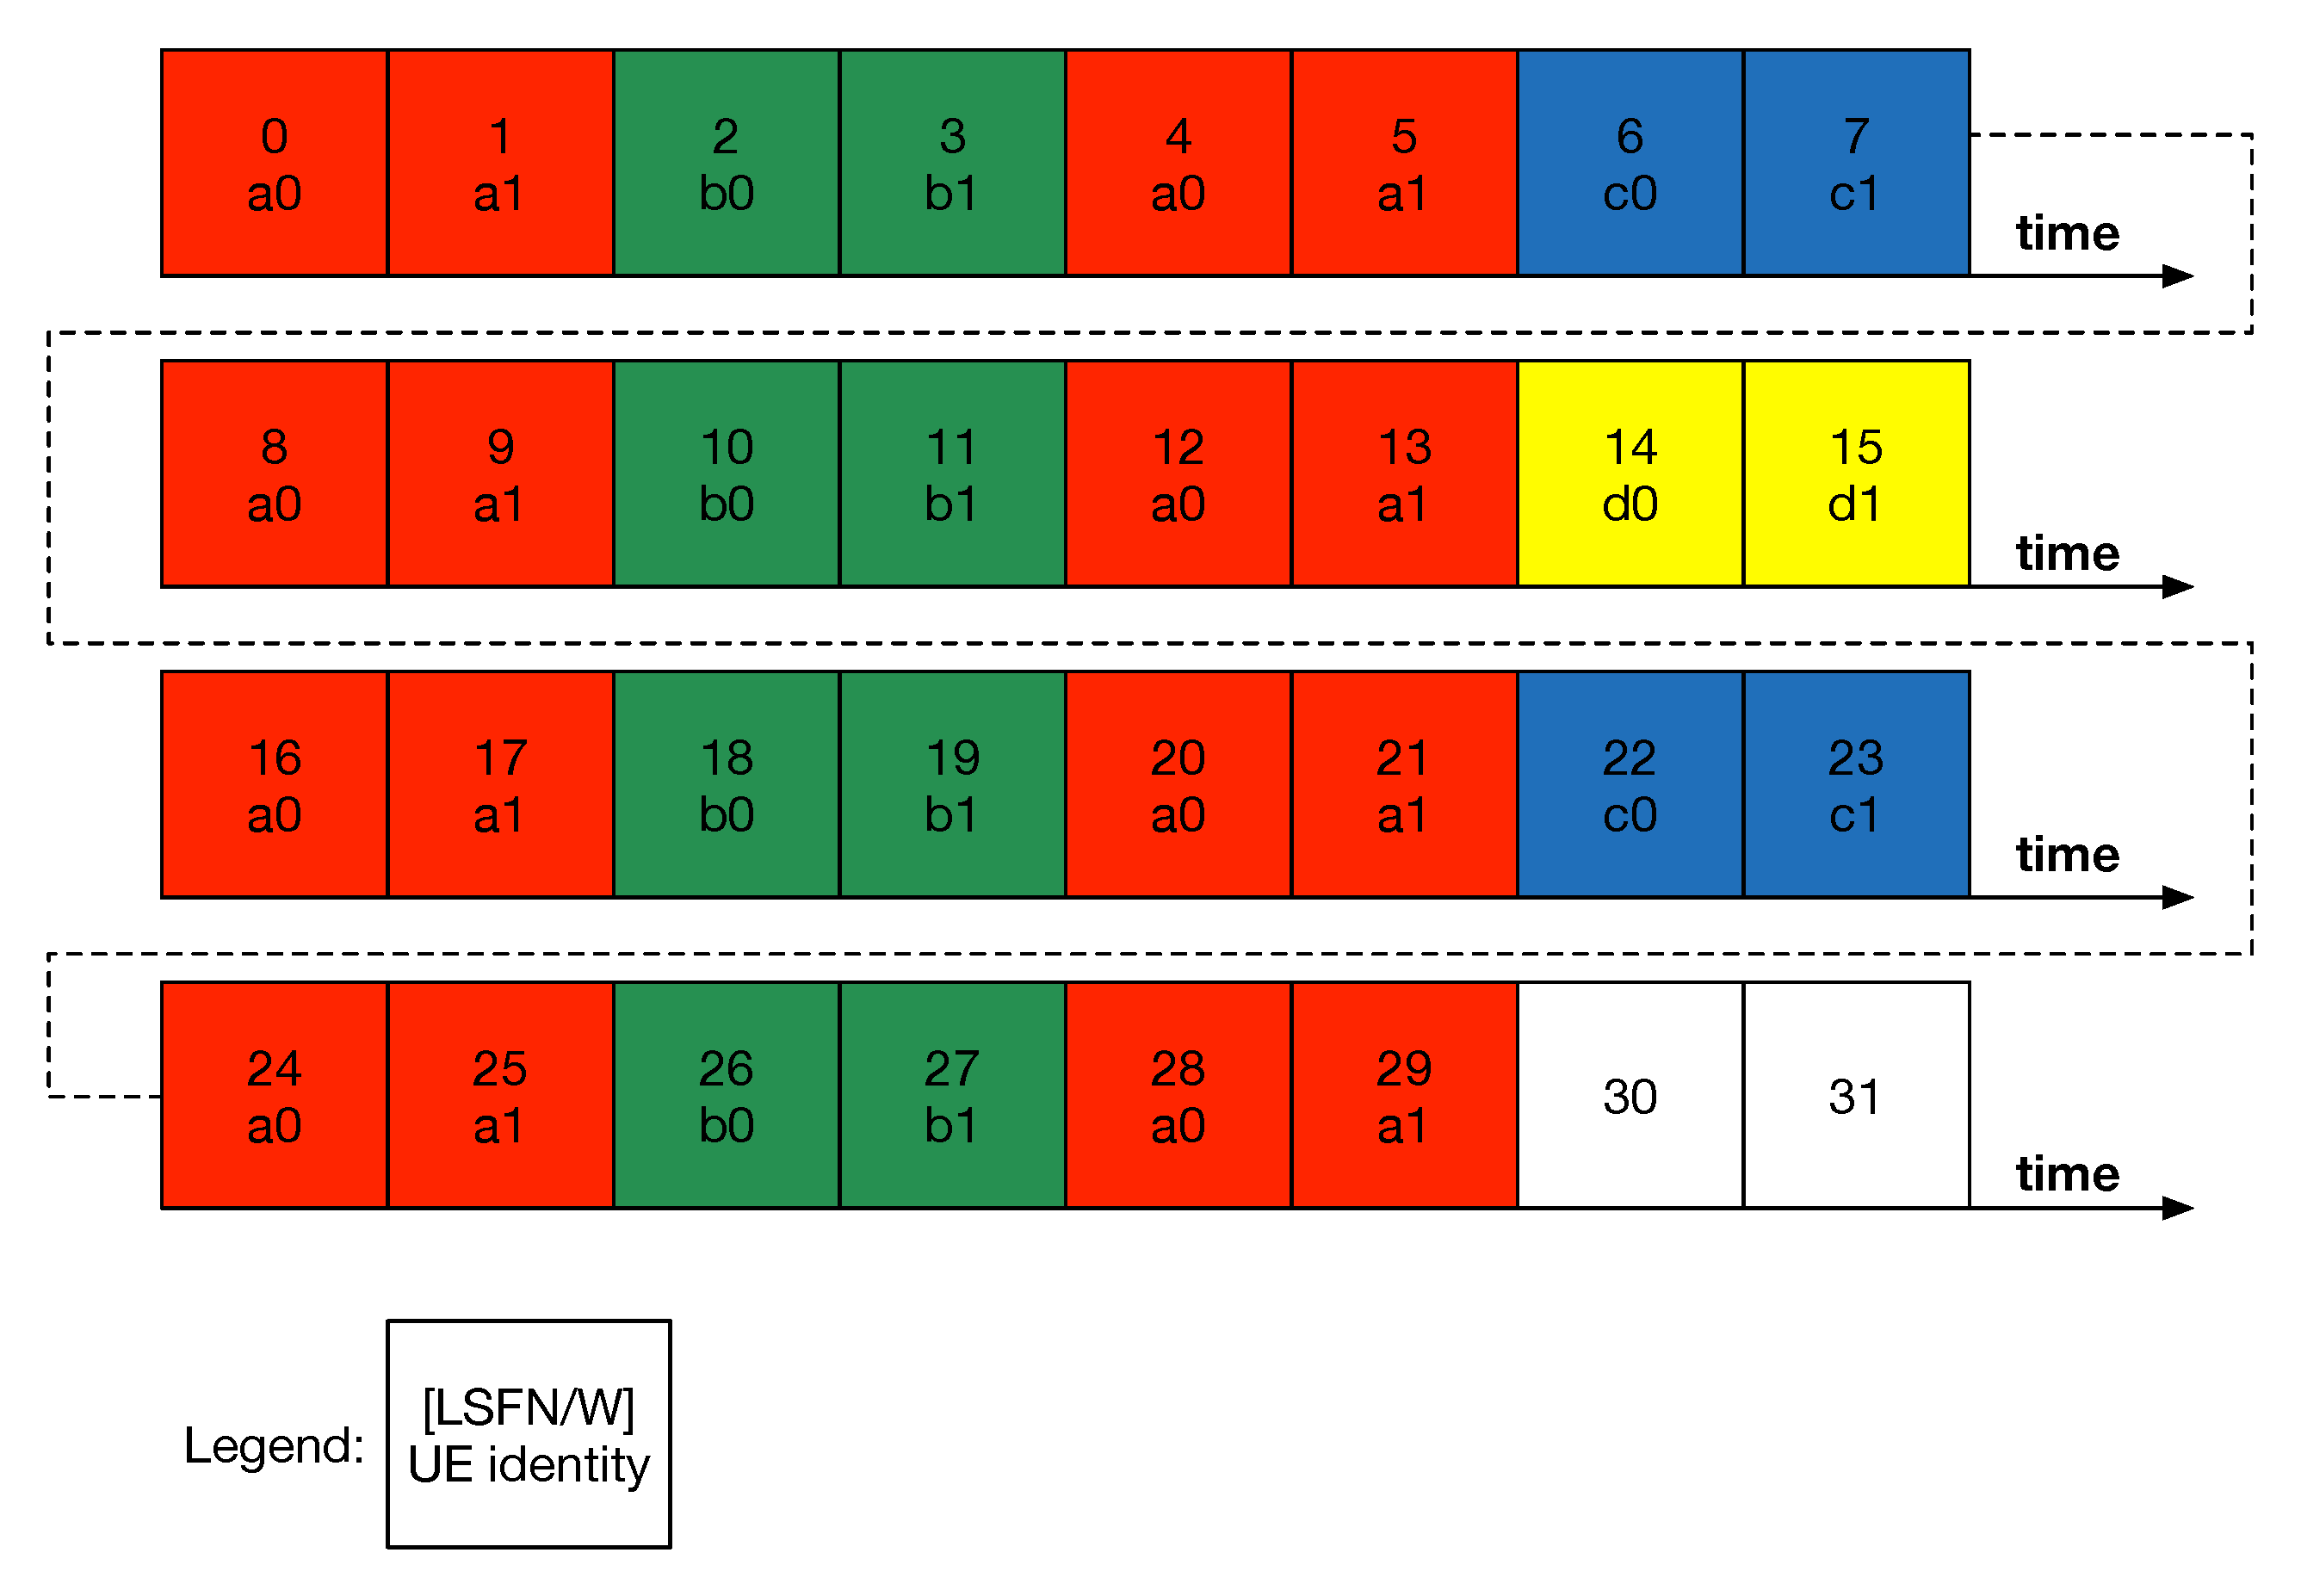
\includegraphics[width=\linewidth]{Chapter6/Figures/Anexampleallocation}
	\caption{Illustration of RNTI allocation result}
	\label{fig:Illustration-Resource-Allocation}
\end{figure}
